\subsection{Transporte de Fluidos}

\subsubsection{Dimensionamento de Tubulações}

Tubulações são componentes por onde o fluido escoa, permitindo a transferência de matéria entre equipamentos, desde a entrada de matéria-prima até a saída de produtos. Seu correto dimensionamento é imprescindível para a segurança e a eficiência do processo.

O dimensionamento consiste em definir o diâmetro nominal e o \textit{schedule} capazes de conduzir as vazões dentro de faixas de velocidade e perda de carga economicamente ótimas. As grandezas envolvidas incluem vazão (mássica ou volumétrica), velocidade admissível, propriedades do fluido (massa específica, viscosidade), comprimento equivalente (devido a acessórios) e características do material (rugosidade, pressão de projeto).

Na prática, calcula-se um diâmetro a partir da vazão e velocidade alvo e seleciona-se o diâmetro comercial imediatamente superior disponível, verificando em seguida a perda de carga pelo método de Darcy–Weisbach e a integridade mecânica conforme normas aplicáveis. Temperatura e pressão afetam propriedades físicas do fluido e critérios de espessura da tubulação; adicionalmente, a topografia da planta e o número de acessórios elevam o comprimento equivalente total.

Subdimensionar uma tubulação implica grandes perdas de carga e custos energéticos; superdimensionar acarreta CAPEX elevado e pode gerar velocidades muito baixas (favorecendo sedimentação em tubulações com sólidos). O embasamento teórico combina a equação de continuidade, correlações de atrito e seleção de materiais, apoiado no uso do diagrama de Moody \cite{white2018}.

\subsubsection{Diâmetro Calculado}

O diâmetro calculado é baseado na vazão e na velocidade média do fluido escoando em um duto circular, de acordo com a Equação \ref{eq:diametro_calc}:

\begin{equation}
D = \sqrt{\frac{4 \cdot Q}{\pi \cdot V}}
\label{eq:diametro_calc}
\end{equation}

Em que:
\begin{itemize}
    \item $Q$ -- vazão volumétrica do fluido;
    \item $V$ -- velocidade média do fluido;
    \item $D$ -- diâmetro hidráulico do duto circular.
\end{itemize}

Essa relação advém diretamente da equação da continuidade para escoamento em regime permanente \cite{white2018}. $Q$ em $\mathrm{m^3/s}$ e $V$ em $\mathrm{m/s}$ dão $D$ em $\mathrm{m}$ na equação; a rotina implementada converte o resultado exibido para $\mathrm{mm}$.

\begin{quote}
\small
\textbf{Pseudocódigo do dimensionamento de diâmetro.}
\begin{verbatim}
receber vazão, velocidade de projeto e unidade
converter vazão para m3/s
calcular área = vazão / velocidade
calcular diâmetro teórico = sqrt(4 * área / pi)
comparar diâmetro teórico com tabela de schedules
retornar diâmetro comercial, velocidade real e critérios de seleção
\end{verbatim}
\end{quote}
\subsubsection{Diâmetro Real}

O diâmetro real corresponde ao diâmetro nominal da tubulação a ser utilizada. Fabricantes produzem tubos em geometrias padronizadas (padrões de espessura como SCH 10, SCH 40, SCH 80 etc.). Deve-se calcular inicialmente o diâmetro necessário pelo método anterior e então escolher, em tabela de catálogo, o tubo comercial com diâmetro interno imediatamente superior, no material e \textit{schedule} desejados. Essa lógica é implementada na função \textit{get\_real\_diameter}, garantindo que o diâmetro selecionado comportará a vazão com velocidade dentro do admissível. Após a seleção, verifica-se a perda de carga resultante e, se necessário, itera-se para outro diâmetro.

\subsubsection{Tubulações}

Para um correto cálculo de perdas de carga e seleção de bombas, o \textit{software} incorpora dados de catálogo de tubulações, rugosidades de materiais e comprimentos equivalentes de acessórios.

\textbf{Rugosidade de materiais.} A rugosidade absoluta do material interno da tubulação influencia o fator de atrito em regime turbulento por meio da rugosidade relativa $\varepsilon/D$. Materiais metálicos, plásticos ou com incrustações apresentam valores típicos de rugosidade tabelados \cite{white2018}. Com o tempo de operação, depósitos e corrosão podem elevar a rugosidade efetiva, devendo-se considerar fatores de segurança.

\textbf{Catálogo de diâmetros.} São armazenadas dimensões padrão de tubulações (diâmetro externo, espessura e diâmetro interno resultante) para diferentes \textit{schedules} (por exemplo, SCH 10, 40 e 80) e materiais. Também podem ser incluídos dados de pressão máxima de trabalho e peso por metro. Isso permite que, dado um diâmetro calculado, o programa selecione o diâmetro nominal comercial mais próximo disponível.

\begin{table}[H]
    \centering
    \caption{Contratos de dados usados no cadastro de tubulações}
    \label{tab:contratos-tubulacoes}
    \small
    \begin{tabular}{>{\raggedright\arraybackslash}p{0.24\textwidth}>{\raggedright\arraybackslash}p{0.28\textwidth}>{\raggedright\arraybackslash}p{0.34\textwidth}}
        \hline
        \textbf{Contrato} & \textbf{Campos principais} & \textbf{Uso no cálculo} \\
        \hline
        Material & nome, rugosidade, descrição & Define propriedades geométricas e hidráulicas associadas à composição da tubulação. \\
        Schedule & diâmetro nominal, diâmetro externo, espessura, diâmetro interno & Seleciona dimensões comerciais para cálculo de velocidade, área e perda de carga. \\
        Acessório & tipo, diâmetro nominal, comprimento equivalente ou coeficiente local & Converte singularidades em contribuição de perda de carga. \\
        \hline
    \end{tabular}
    \fonte{Autoria própria.}
\end{table}

\textbf{Coeficientes de perda em acessórios.} Curvas, válvulas, expansões, contrações e conexões diversas introduzem perdas de carga locais. No modelo implementado, cada acessório pode ser contabilizado por um comprimento equivalente $L_{eq}$ ou por um fator adimensional de perda $K$. O comprimento equivalente total da tubulação é obtido pela soma dos acessórios e acrescentado ao comprimento linear. Esses dados, como fatores $K$ ou $L_{eq}$ típicos para cada acessório padrão, foram compilados de literatura de engenharia de escoamento \cite{perry2007}.

No cálculo de perdas de carga totais, o comprimento $L$ da tubulação reta é acrescido do comprimento equivalente $\sum_{}^{} L_{eq}$ das singularidades presentes. Uma estimativa inadequada da rugosidade ou do efeito de acessórios pode produzir erros significativos na previsão de perda de carga, resultando em superdimensionamento ou subdimensionamento de bombas. Assim, o uso de dados acurados de catálogo e correlações de atrito é fundamental para a confiabilidade do dimensionamento. A Tabela a seguir resume o fluxo do cálculo de perda de carga por Darcy--Weisbach utilizando acessórios.

\begin{table}[H]
    \centering
    \caption{Fluxo de cálculo da perda de carga com acessórios}
    \label{tab:fluxo-perda-carga-acessorios}
    \small
    \begin{tabular}{p{0.25\textwidth}p{0.57\textwidth}}
        \hline
        \textbf{Etapa} & \textbf{Operação e verificação} \\
        \hline
        Entradas & Método, fator de atrito, comprimento, diâmetro, velocidade ou vazão e acessórios. \\
        Preparação & Converte as grandezas para unidades coerentes e soma os comprimentos equivalentes das singularidades. \\
        Processamento & Aplica Darcy--Weisbach ou Hazen--Williams conforme o método selecionado. \\
        Saída e validação & Retorna a perda de carga em metros e rejeita entradas ausentes, não numéricas ou resultados não positivos. \\
        \hline
    \end{tabular}
    \fonte{Autoria própria.}
\end{table}


\subsubsection{Escoamento, Perdas de Carga e Diâmetros Hidráulicos}

O comportamento do escoamento interno é governado, principalmente, pelo número de Reynolds, que permite classificar o regime como laminar, de transição ou turbulento. Variáveis-chave incluem o diâmetro hidráulico, a velocidade média, a viscosidade e a massa específica do fluido, bem como a rugosidade relativa da parede. Perfis de velocidade, mecanismos de mistura e dissipação de energia por atrito dependem desse regime de escoamento. Para quantificar a perda de carga (queda de pressão) devida ao atrito no escoamento, emprega-se a equação universal de Darcy–Weisbach \cite{white2018}.

No regime turbulento, o fator de atrito $f$ depende de $Re$ e da rugosidade relativa $\varepsilon/D$, não possuindo solução analítica explícita; por isso, utilizam-se relações empíricas ou aproximadas. Já no regime laminar ($Re < 2300$), o perfil de velocidades é parabólico e $f$ admite a expressão simples dada pela Equação \ref{eq:laminar_friction}:
\begin{equation}
f = \frac{64}{Re}
\label{eq:laminar_friction}
\end{equation}.

Em serviços de água a escoamento turbulento, a fórmula empírica de Hazen--Williams é comumente empregada como aproximação prática \cite{perry2007}. Temperatura e pressão afetam massa específica e viscosidade do fluido, modificando o valor de $Re$ e, consequentemente, as perdas de carga.

Além disso, o material e condições da tubulação (nova, envelhecida) determinam a rugosidade efetiva. Todos esses efeitos impactam diretamente o balanço de energia no escoamento em tubulações e a potência requerida em bombas ou compressores \cite{perry2007,white2018}.

\begin{table}[H]
    \centering
    \caption{Unidades e natureza dos grupos de Reynolds e fator de atrito}
    \label{tab:unidades-reynolds-atrito}
    \begin{tabular}{|p{0.30\textwidth}|p{0.60\textwidth}|}
        \hline
        \textbf{Símbolo} & \textbf{Unidade ou natureza} \\ \hline
        $Re$ & Número de Reynolds adimensional. \\ \hline
        $f$ & Fator de atrito de Darcy adimensional. \\ \hline
        $D$ & Diâmetro da tubulação em unidade de comprimento, por exemplo $\mathrm{m}$. \\ \hline
        $\rho$ & Massa específica, por exemplo $\mathrm{kg/m^3}$. \\ \hline
        $V$ & Velocidade média, por exemplo $\mathrm{m/s}$. \\ \hline
        $\mu$ & Viscosidade dinâmica, por exemplo $\mathrm{Pa\,s}$. \\ \hline
        $\nu$ & Viscosidade cinemática, por exemplo $\mathrm{m^2/s}$. \\ \hline
        $\varepsilon$ & Rugosidade absoluta na mesma unidade de comprimento usada para $D$. \\ \hline
        $\varepsilon/D$ & Rugosidade relativa adimensional. \\ \hline
    \end{tabular}
\end{table}

\subsubsection{Número de Reynolds}

O número de Reynolds ($Re$) relaciona as forças inerciais com as forças viscosas no escoamento dentro de uma tubulação:

Usando viscosidade dinâmica $\mu$:
\begin{equation}
Re = \frac{D \cdot V \cdot \rho}{\mu}
\label{eq:reynolds_din}
\end{equation}

Usando viscosidade cinemática $\nu$:
\begin{equation}
Re = \frac{D \cdot V}{\nu}
\label{eq:reynolds_cin}
\end{equation}

Com esses símbolos padronizados, tipicamente $Re < 2300$ indica regime laminar, $2300 < Re < 4000$ indica regime de transição, e $Re > 4000$ indica regime turbulento plenamente desenvolvido \cite{white2018}.

\begin{quote}
\small
\textbf{Fluxo de cálculo do número de Reynolds.}
\begin{verbatim}
receber diâmetro característico e velocidade
selecionar viscosidade dinâmica com massa específica
ou viscosidade cinemática
converter grandezas para unidades coerentes
calcular Re = D * V * rho / mu ou Re = D * V / nu
classificar regime e retornar número de Reynolds positivo
\end{verbatim}
\end{quote}

\subsubsection{Fator de Atrito}

No regime laminar, o fator de atrito de Darcy pode ser obtido diretamente por $f = 64/Re$. No regime turbulento, $f$ satisfaz implicitamente a equação de Colebrook--White \cite{colebrook1939}:

\begin{equation}
\frac{1}{\sqrt{f}} = -2 \log_{10} \left( \frac{\varepsilon}{3{,}7D_{h}} + \frac{2{,}51}{Re\sqrt{f}} \right)
\label{eq:colebrook}
\end{equation}

A rugosidade relativa captura o efeito da parede no regime turbulento. Para evitar a resolução iterativa, existem correlações explícitas aproximadas amplamente usadas, por exemplo:

Swamee--Jain \cite{swamee1976}:

\begin{equation}
f = \frac{0{,}25}{\left[\log_{10}\left( \frac{\varepsilon}{3{,}7D} + \frac{5{,}74}{Re^{0{,}9}} \right)\right]^2}
\label{eq:swamee}
\end{equation}

Haaland \cite{haaland1983}:

\begin{equation}
\frac{1}{\sqrt{f}} = -1{,}8 \log_{10} \left[ \left(\frac{\varepsilon/D}{3{,}7}\right)^{1{,}11} + \frac{6{,}9}{Re} \right]
\label{eq:haaland}
\end{equation}

O \textit{software} implementa as equações acima para cálculo de $f$ conforme o regime e dados disponíveis \cite{white2018}. A interface para a obtenção do fator de atrito e as opções disponibilizadas ao usuário estão exibidas na Figura \ref{fig:friction_factor_calc}.

\begin{figure}[H]
    \centering
    \caption{Interface de cálculo do fator de atrito}
    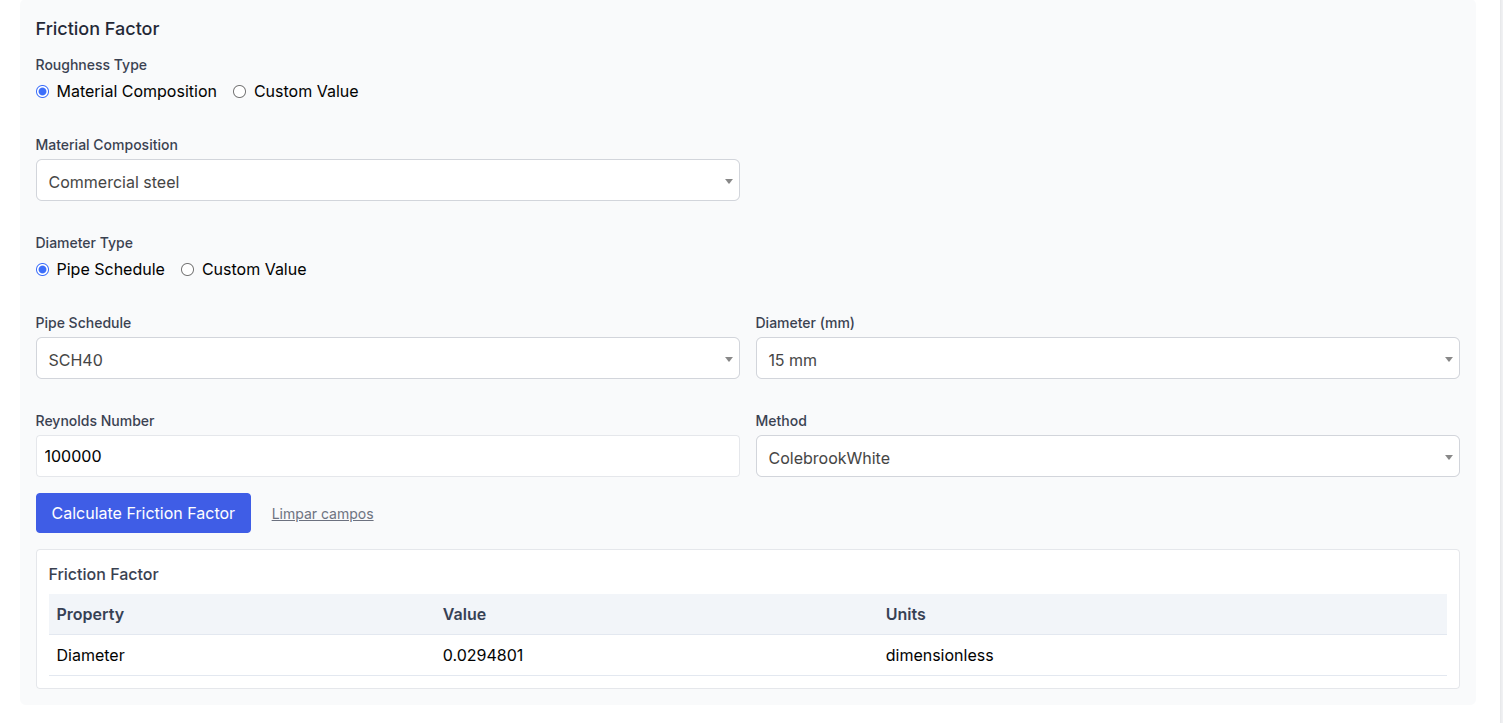
\includegraphics[width=\linewidth]{media/cap4_diagrama_moody.png}
    \fonte{Elaboração própria (2026).}
    \label{fig:friction_factor_calc}
\end{figure}

\begin{quote}
\small
\textbf{Fluxo de cálculo do fator de atrito.}
\begin{verbatim}
receber rugosidade, diâmetro, Reynolds e método
calcular rugosidade relativa
se método = ColebrookWhite, resolver a equação implicitamente
se método = SwameeJain ou Haaland, aplicar a correlação explícita
retornar fator de atrito adimensional ou erro de convergência
\end{verbatim}
\end{quote}

\subsubsection{Perda de Carga -- Darcy--Weisbach e Hazen--Williams}

A perda de carga distribuída $h_{f}$ em uma tubulação de comprimento $L$ é calculada pela equação de Darcy–Weisbach:

\begin{equation}
h_{f} = f \cdot \frac{\left( L + \sum_{}^{} L_{e q} \right)}{D} \frac{V^{2}}{2 g}
\label{eq:darcy}
\end{equation}

Na Equação \ref{eq:darcy}, $h_f$, $L$, $\sum L_{eq}$ e $D$ usam unidades de comprimento coerentes; $V$ é velocidade, por exemplo $\mathrm{m/s}$; $g$ é aceleração, por exemplo $\mathrm{m/s^2}$; e $f$ é adimensional. O resultado de $h_f$ é uma altura de perda de carga, usualmente expressa em $\mathrm{m}$. Essa fórmula é universal e independe do fluido, desde que $f$ seja adequadamente determinado \cite{perry2007}.

Para escoamento de água em tubulações de diâmetro moderado (tipicamente $D > 50\ \mathrm{mm}$) e regime turbulento plenamente estabelecido, a fórmula empírica de Hazen--Williams pode ser empregada como simplificação:

\begin{equation}
h_{f} = \frac{4{,}73 L}{C^{1{,}852}D^{4{,}87}} Q^{1{,}852}
\label{eq:hazen}
\end{equation}

Na forma exibida, o coeficiente empírico $4{,}73$ corresponde à convenção inglesa usual da correlação, com $h_f$ e $L$ em pés, $Q$ em $\mathrm{ft^3/s}$ e $D$ em pés; portanto, as unidades devem seguir a convenção associada ao coeficiente. Quando se usa a forma SI, com $h_f$ e $L$ em $\mathrm{m}$, $Q$ em $\mathrm{m^3/s}$ e $D$ em $\mathrm{m}$, o coeficiente empírico muda. Em ambas as formas, $C$ é o coeficiente de Hazen--Williams do material, tratado como adimensional e tabelado para tubulações novas de ferro fundido, aço, PVC etc. Apesar de não possuir fundamentação teórica geral, essa equação fornece boa precisão para água a 20\,°C em tubulações de transporte e é consagrada no projeto de redes de água devido à sua simplicidade \cite{perry2007,white2018}.

\begin{quote}
\small
\textbf{Fluxo de cálculo da perda de carga.}
\begin{verbatim}
receber método, geometria, vazão ou velocidade e propriedades da tubulação
resolver a velocidade ou a vazão faltante quando necessário
somar comprimento reto e comprimentos equivalentes
aplicar Darcy-Weisbach ou Hazen-Williams
retornar perda de carga em metros e validar sinal e faixa de aplicação
\end{verbatim}
\end{quote}


\subsubsection{Diâmetro Hidráulico para Geometrias Diversas}

O conceito de diâmetro hidráulico generaliza o cálculo do número de Reynolds e do fator de atrito para seções transversais não circulares. O diâmetro hidráulico é definido como:
\begin{equation}
D_{h} = \frac{4 A}{P}
\label{eq:diametro_hidraulico}
\end{equation}
onde $A$ é a área da seção transversal de escoamento e $P$ o perímetro molhado (contorno em contato com o fluido). Assim:

Para dutos circulares, conforme a Equação \ref{eq:dh_circular}:
\begin{equation}
D_{h} = D
\label{eq:dh_circular}
\end{equation}
(recupera o diâmetro interno). Para canais ou abertos, conforme a Equação \ref{eq:dh_rect}:
\begin{equation}
D_{h} = \frac{4 a b}{2 ( a + b )}
\label{eq:dh_rect}
\end{equation}
onde $a$ e $b$ são os lados do retângulo. Para anulares (espaço entre dois tubos concêntricos), conforme a Equação \ref{eq:dh_annular}:
\begin{equation}
D_{h} = D_{o} - D_{i}
\label{eq:dh_annular}
\end{equation}
(diferença entre diâmetro externo interno e diâmetro externo do interno). Para seções triangulares (por ex., condutos abertos triangulares), calcula-se $A$ e $P$ conforme a geometria e aplica-se $4 A / P$. Para geometrias mais complexas (ex.: calhas semicirculares), também se aplica $4 A / P$ considerando o perímetro molhado adequadamente.

Nas Equações \ref{eq:diametro_hidraulico} a \ref{eq:dh_annular}, $D_h$, $D$, $D_o$, $D_i$, $a$, $b$ e o perímetro molhado $P$ (ou $P_m$) usam a mesma unidade de comprimento; $A$ usa a unidade de área correspondente; e cada fórmula retorna $D_h$ nessa unidade de comprimento.

\begin{figure}[H]
    \centering
    \caption{Tipos de dutos de escoamento}
    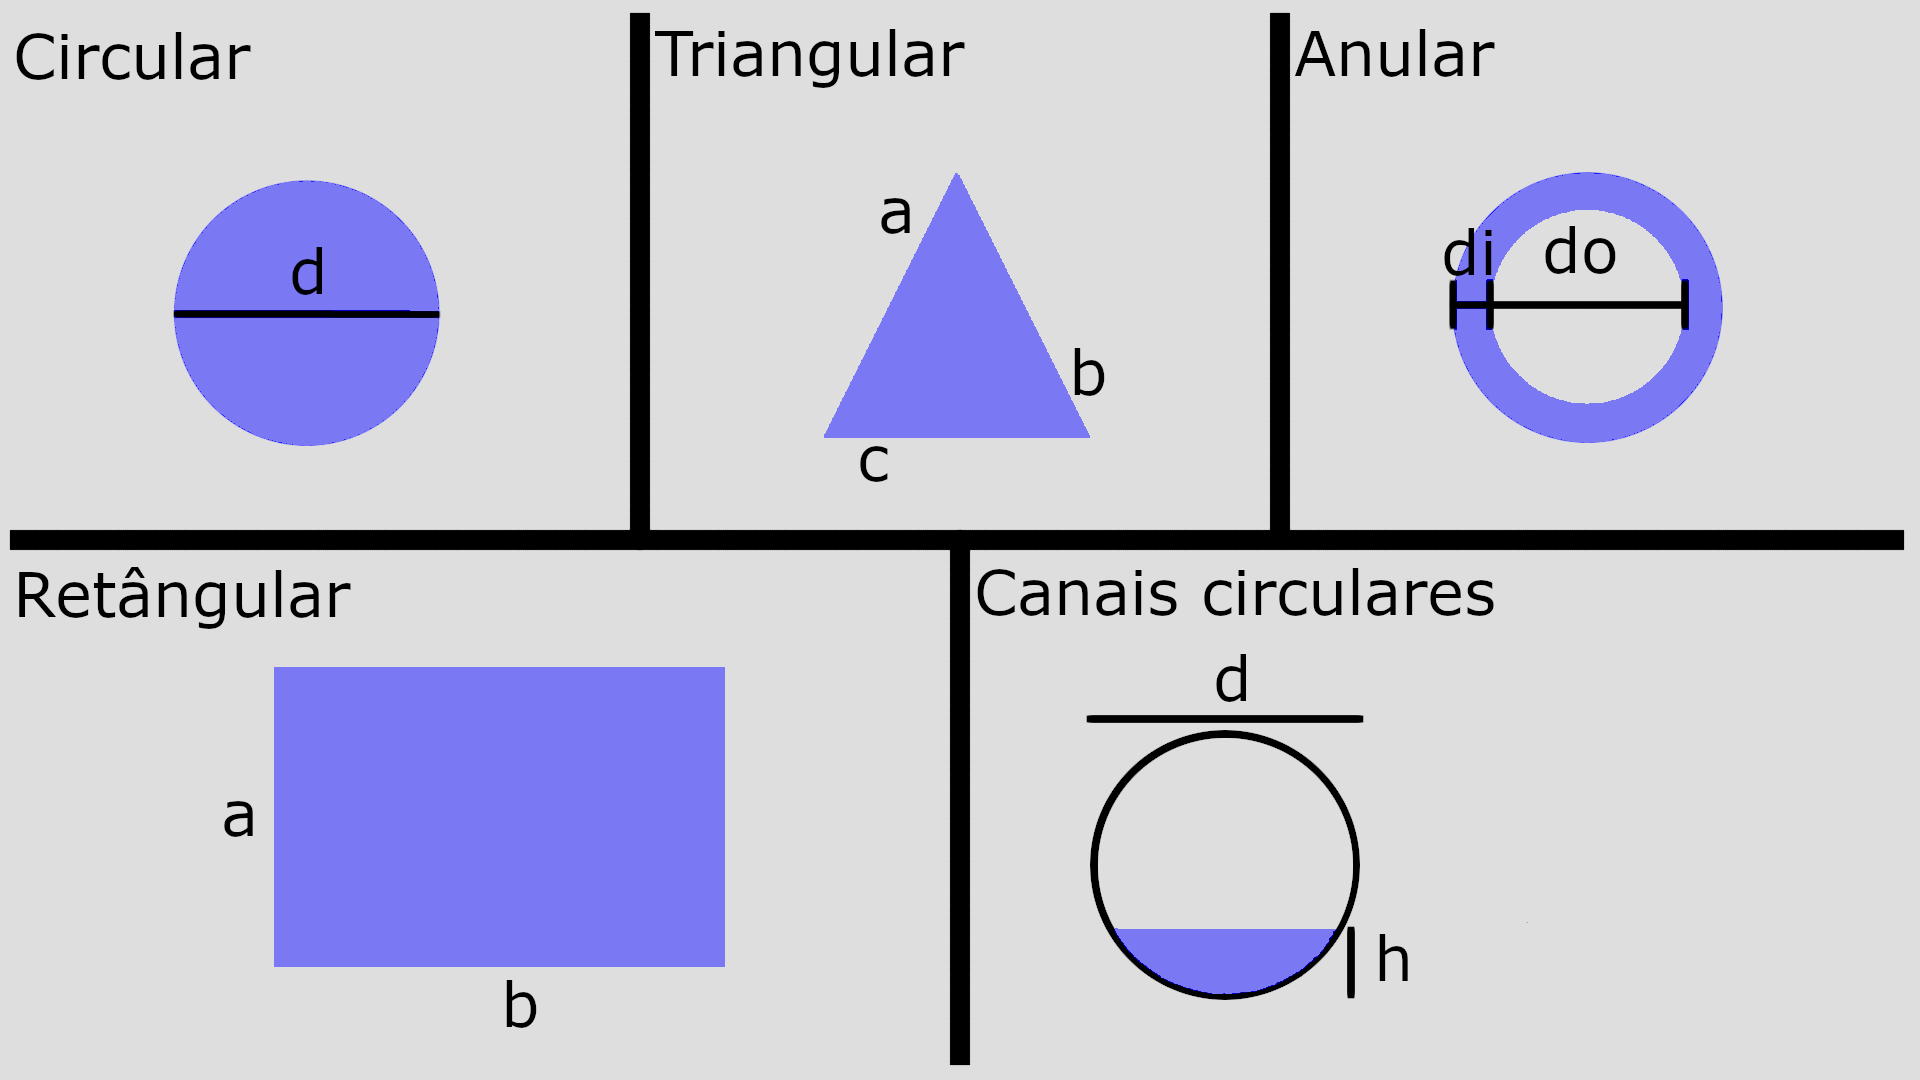
\includegraphics[width=\linewidth]{media/cap4_tipos_dutos_escoamento.png}
    \fonte{Elaboração própria (2026).}
\end{figure}

O programa permite ao usuário informar $A$ e $P$ para cálculo de $D_{h}$ em situações especiais, garantindo flexibilidade para tratar geometrias arbitrárias \cite{white2018}.

\begin{quote}
\small
\textbf{Fluxo de cálculo do diâmetro hidráulico.}
\begin{verbatim}
receber geometria e dimensões específicas da seção
calcular área e perímetro molhado conforme a geometria
aplicar Dh = 4 * área / perímetro
validar dimensões, desigualdade triangular ou altura do segmento
retornar diâmetro hidráulico na unidade de entrada
\end{verbatim}
\end{quote}
